\documentclass{article}

% if you need to pass options to natbib, use, e.g.:
% \PassOptionsToPackage{numbers, compress}{natbib}
% before loading nips_2017
%
% to avoid loading the natbib package, add option nonatbib:
% \usepackage[nonatbib]{nips_2017}

\usepackage[final]{nips_2017}

% to compile a camera-ready version, add the [final] option, e.g.:
% \usepackage[final]{nips_2017}

\usepackage[utf8]{inputenc} % allow utf-8 input
\usepackage[T1]{fontenc}    % use 8-bit T1 fonts
\usepackage{hyperref}       % hyperlinks
\usepackage{url}            % simple URL typesetting
\usepackage{booktabs}       % professional-quality tables
\usepackage{amsfonts}       % blackboard math symbols
\usepackage{nicefrac}       % compact symbols for 1/2, etc.
\usepackage{microtype}      % microtypography
\usepackage{graphicx}

\title{CNN Assistance in Jigsaw Puzzle Solution}

% The \author macro works with any number of authors. There are two
% commands used to separate the names and addresses of multiple
% authors: \And and \AND.
%
% Using \And between authors leaves it to LaTeX to determine where to
% break the lines. Using \AND forces a line break at that point. So,
% if LaTeX puts 3 of 4 authors names on the first line, and the last
% on the second line, try using \AND instead of \And before the third
% author name.

\author{Tianbao Li\\
  Department of Computer Science\\
  University of Toronto\\
  Toronto, ON M5S 1A1 \\
  \texttt{tianbao@cs.toronto.edu} \\
  %% examples of more authors
  %% \And
  %% Coauthor \\
  %% Affiliation \\
  %% Address \\
  %% \texttt{email} \\
  %% \AND
  %% Coauthor \\
  %% Affiliation \\
  %% Address \\
  %% \texttt{email} \\
  %% \And
  %% Coauthor \\
  %% Affiliation \\
  %% Address \\
  %% \texttt{email} \\
  %% \And
  %% Coauthor \\
  %% Affiliation \\
  %% Address \\
  %% \texttt{email} \\
}

\begin{document}
% \nipsfinalcopy is no longer used

\maketitle

\begin{abstract}

This paper presents an innovative way to assist solving jigsaw puzzle with the help of deep convolutional neural networks. The main goal of this project is to predict whether two pieces from the jigsaw puzzleshould be neighbors in the origin image. Proceeding from traditional methods of using color (like RGB) diastance, here, we introduce the low level features in the image which are extracted by convolutional neural networks. Compared with color-based solutions, using the feature maps generated can help with a deeper intuition on the correlation between edges. The proposed algorithm can achieve considerable accuracy on adjacency prediction.

\end{abstract}

\section{Introduction}

Jigsaw puzzles were first introduced around 1760 for map research and then became a popular intelligence entertainment \cite{freeman1964apictorial} in the last few centuries. The origin image is divided into $N\times M$. To solve htis, people need to cluster similar tiles, find the neighbors and then reconstruct the origin image. However, due to the possible locations and relationship behind pieces, there are quite a huge number of sulotions ever for a small jigsae puzzle, for example, $(8*8)!=1.2688693*10^{89}$ solutions for an $8*8$ puzzle. Indeed, this problem has be proven to be a NP-complete one \cite{altman1989solving,demaine2007jigsaw}. Though tough, actually, jigsaw puzzle solving is quite meaningful beyond the intelligence challenge. It helps a lot in combining shredded of documents \cite{levin1975computer,marques2009reconstructing} and even recovering artifacts debris\cite{koller2006computer}.

Recently year, there have been a lot researchers working on this problem and achieved much progress. However, one the the most important sub-problems in this procedure, determining adjancency between pieces, seems keeps in the same track for long. When people solve the puzzle manually, they need needs image information at edges, such as color, texture, instance, etc. to make the judgement whether two pieces are neighbors. However, most of previous research only eyes on the color features such as RGB distance. This make such solutions quite bad for simple-colored images, especially in reconstructing printed documents ot ancient artifacts.

Here, we want to mimic how people really solve jigsaw puzzles and work on finding features capable to help make adjancent prediction. Recently, Concolution Neural Networks (CNN) leads the research area of computer vision with its capability of extracting inside features underneath the images and sole hard problems such as detection\cite{redmon2017yolo9000} and segmentation\cite{he2017mask,yu2015multi}. Based on the existing tremendous structures, people start to apply transfer learning and use extracted features to solve related computer vision problems\cite{razavian2014cnn}.

In this paper, we contribute in providing neural networks to predict whether two tiles from a jigsaw puzzle are adjancent in the origin image. The neural networks judge the jigsaw piece pair by extracted low lever image features from pre-trained CNN together with color information at edges, and outputs whether this two tiles are neighbors. This model achieves outstanding prediction accuracy in images from ILSVRC2012 dataset\cite{ILSVRC15}.

\section{Related Work}

Jigsaw has been researched on for many years. One most basic idea is to evaluate the compatibility of the adjacent pieces and take a strategy, such as greedy search, to arrange the pieces. One famous work is the Genetic Algorithm (GA) \cite{sholomon2013genetic}. Given initial candidate solutions, it applies operations like selection, reproduction and mutation based on the color-distance fitness function. Similarly but innovatively, \cite{sholomon2016dnn} first introduces deep neural network to jigsaw solver and transforms the puzzle to the piece pair adjacency prediction. It samples piece edges to learn the adjacent likelihood through DNN based on the color distance. For these two solvers, they only use color information to judge whether two pieces should be together. However, human use some others like texture to solve. Also, though high accuracy, these solution could not solve the jigsaw puzzle whici generated by single-colored or colerless images. So, there are still some further steps on it.

Recently, with the prosper of convolutional neural networks in computer vision area, convolutional neural networks (CNN) also becomes a good tool to solve jigsaw puzzles. Because of the fact that a good CNN is hard to train and the training data needs many images and well labels, more and more researchers choose the apply transfer learning on pre-trained models, fine turning on the last a few layers or using it as a feature extractor, instead of go over all the process \cite{razavian2014cnn}. CNN can extract regional features in many perspectives, such as color, texture, pattern, instance. Features in the formers usually reflect the basic information of the images, while the latter layers can make high-level judgement. These can be good inference for judging adjacent pieces. So, \cite{deryneural,noroozi2016unsupervised} choose to use feature maps from pre-trained CFN \cite{noroozi2016unsupervised} (siamese-ennead AlexNet \cite{krizhevsky2012imagenet}), VGG \cite{he2016deep} or Resnet \cite{simonyan2014very} and predict the location. However, the main problem for these approach is that they hold a siamese structure with shared weights for each location, which means they can only solve a limited number for pieces ($3\times3$ in \cite{noroozi2016unsupervised}, $2\times2$ and $2\times3$ in \cite{deryneural}). With the piece amount increasing, the network becomes extremely heavy to train.

\section{preliminary}

\subsection{Problem Definition}

Jigsaw puzzles aims to reshape multiple non-overlapping pieces from the origin image to the correct arrangement. In our project, like in most computer research, we focus on equal-sized squared $W=N\times M$ pieces. It refuses the aid of shape matching but asks for more on image information. The expected result is a set of indexes $I=(p_1,p_2,\dots,p_W)$ which $p_i$ is the corresponding index for each piece in the origin image. For the worst case, it takes the complicity of $O(W!)$. For example, Figure~\ref{fig:jigsawpuzzleexample} is a $3*3$ jigsaw puzzle. The left subgraph is the origin image, and the right subgraph is the puzzle which $I=\{6,2,7,3,5,4,0,8,1\}$.

\begin{figure}
  \begin{minipage}{.50\textwidth}
    \centering
    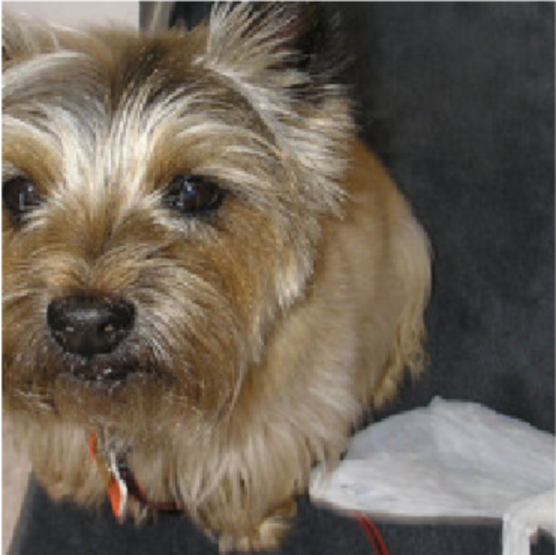
\includegraphics[width=2.5in]{origin_color}
  \end{minipage}
  \begin{minipage}{.50\textwidth}
    \centering
    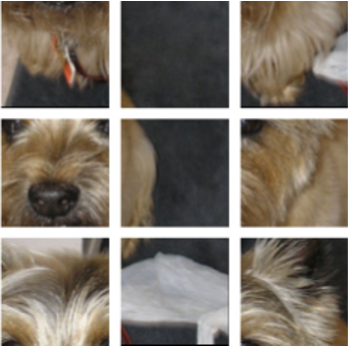
\includegraphics[width=2.5in]{puzzle_color}
  \end{minipage}
  \caption{Jigsaw Puzzle Example}
  \label{fig:jigsawpuzzleexample}
\end{figure}


\bibliographystyle{plain}
\bibliography{Jigsaw-Puzzle-Solver}

\end{document}
